\chapter{Results}


This chapter discribe and illustrate the results generated from the system. In the chapter, section \ref{sec:ExperimentsSetup} will describe the experiments performed on each block of the system. section \ref{sec:Datasets} will describe the datasets used. Section \ref{sec:ResultsDetails} will demonstrate and analysis the result generated. 

\section{Experiments Setup}
\label{sec:ExperimentsSetup}
The system was tested using various experiments. The preprocessing procedures and computation was tested by its effects on the segmentation algorithm and was reported in section (\ref{sec:ResultsDetails}). The variable used to tune the swarm algorithm were tested to choose the best parameters to use(see section \ref{sec:PSO}). Segmentation algorithms test was reported and noted in section \ref{sec:SegmentationAlgorithms}. 

\section{Datasets}
\label{sec:Datasets}
For classifier and algorithm testing the system used a data set collected by \citeauthor{HeloiseBeautification}. The data are drawn by 16 users each of them have drawn from 30 to 50 samples for each shape. Figure \ref{fig:symbolSet} shows the shapes used in the data set. We divided the dataset equally into training set and test set.  The results displayed are the recognition accuracy resulted from the classifier after recognizing the symbols. \\
%We divided the dataset into four sets each set contains four different users. Furthermore, each set is divided into train and test set where the trained set where used to train the classifiers and the test set where used for testing.  The algorithms are then tested using the four sets and the results are averaged.
\begin{figure}[]\centering
\fbox{  \parbox{8cm}{% 
		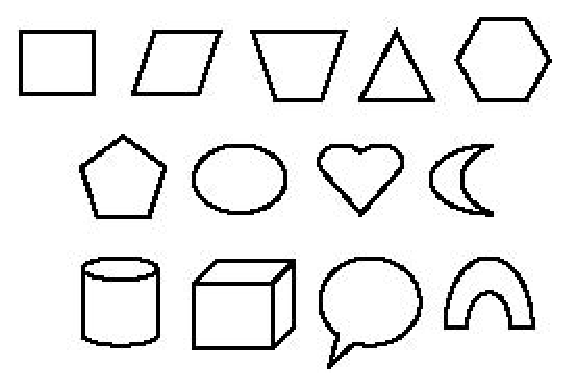
\includegraphics[scale=0.7]{images/symbolSet.eps}	}
		}
	\caption{The Symbol Set}
	\label{fig:symbolSet}
\end{figure}



%\section{Evaluations techniques}
%\label{sec:EvaluationsTechniques}
%\section {Curvature estimation results}
%\label{sec:Curvatureestimationresults}


\section{Results}
\label{sec:ResultsDetails}

\subsection{PSO Algorithm}
\label{sec:PSO}
The fig. \ref{fig:dataerrorvsiteration.jpg} display the effect of the size of swarm population on the number of vertex reported while segmenting the stroke.\footnote{The fewer the vertex the better the segmentation} The graphs shows that as the number of iteration increase there is a decrease in error until the error reach a saturation and any increase in number of iteration dose not affect the error calculated. Similar behavior is noticed in fig. \ref{fig:datapopulation.jpg}.  These curves and test result in choosing the swarm parameters $c_1,c_2$ and maximum number of iteration and the swarm population. The final values are for maximum number of iteration = 150 with 15 particle for better compensation in the time domain. 

\begin{figure}
	\centering
		\includegraphics[scale=0.8]{images/dataerrorvsiteration.jpg.eps}
	\caption{Error vs. iterations }
	\label{fig:dataerrorvsiteration.jpg}
\end{figure}
\begin{figure}
	\centering
		\includegraphics[scale=0.8]{images/datapopulation.jpg.eps}
	\caption{Swarm Population }
	\label{fig:datapopulation.jpg}
\end{figure}


\subsection{Segmentation Algorithms}
\label{sec:SegmentationAlgorithms}
The result of the segmentation algorithm can be viewed in the figs. \ref{fig:results1.JPG}. These result shows the originals stroke and the segmentation that the system generated for the stroke. 
\begin{figure}
	\centering
		\includegraphics{images/results1.JPG.eps}
	\caption{Results Segmentations}
	\label{fig:results1.JPG}
\end{figure}
\begin{figure}
	\centering
		\includegraphics{images/results2.JPG.eps}
	\caption{Results Segmentaion }
	\label{fig:results2.JPG}
\end{figure}
\begin{figure}
	\centering
		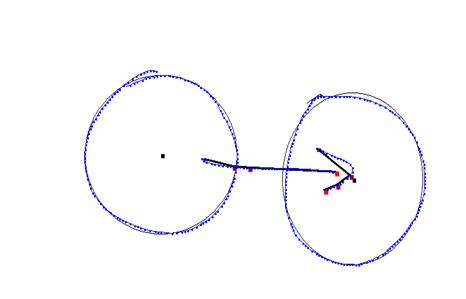
\includegraphics{images/results3.JPG.eps}
	\caption{Results }
	\label{fig:results3.JPG}
\end{figure}
\begin{figure}
	\centering
		\includegraphics{images/results4.JPG.eps}
	\caption{Resluts of the segmentations}
	\label{fig:results4.JPG}
\end{figure}



The experiment we implemented was to test the effect of symbol complexity and type on the recognition rate. Figure \ref{fig:test2} shows what the accuracy of each symbol, it clearly noted that symbols that have only line segments achieve higher accuracy rate than other symbols. Figure \ref{fig:test2} also shows that algorithm 1 alone achieve better performance than algorithm 2 in the symbols that consist of lines only. The combining of both algorithm improves the recognition rate of other symbols.  \\
\begin{figure*}[]
	\centering
		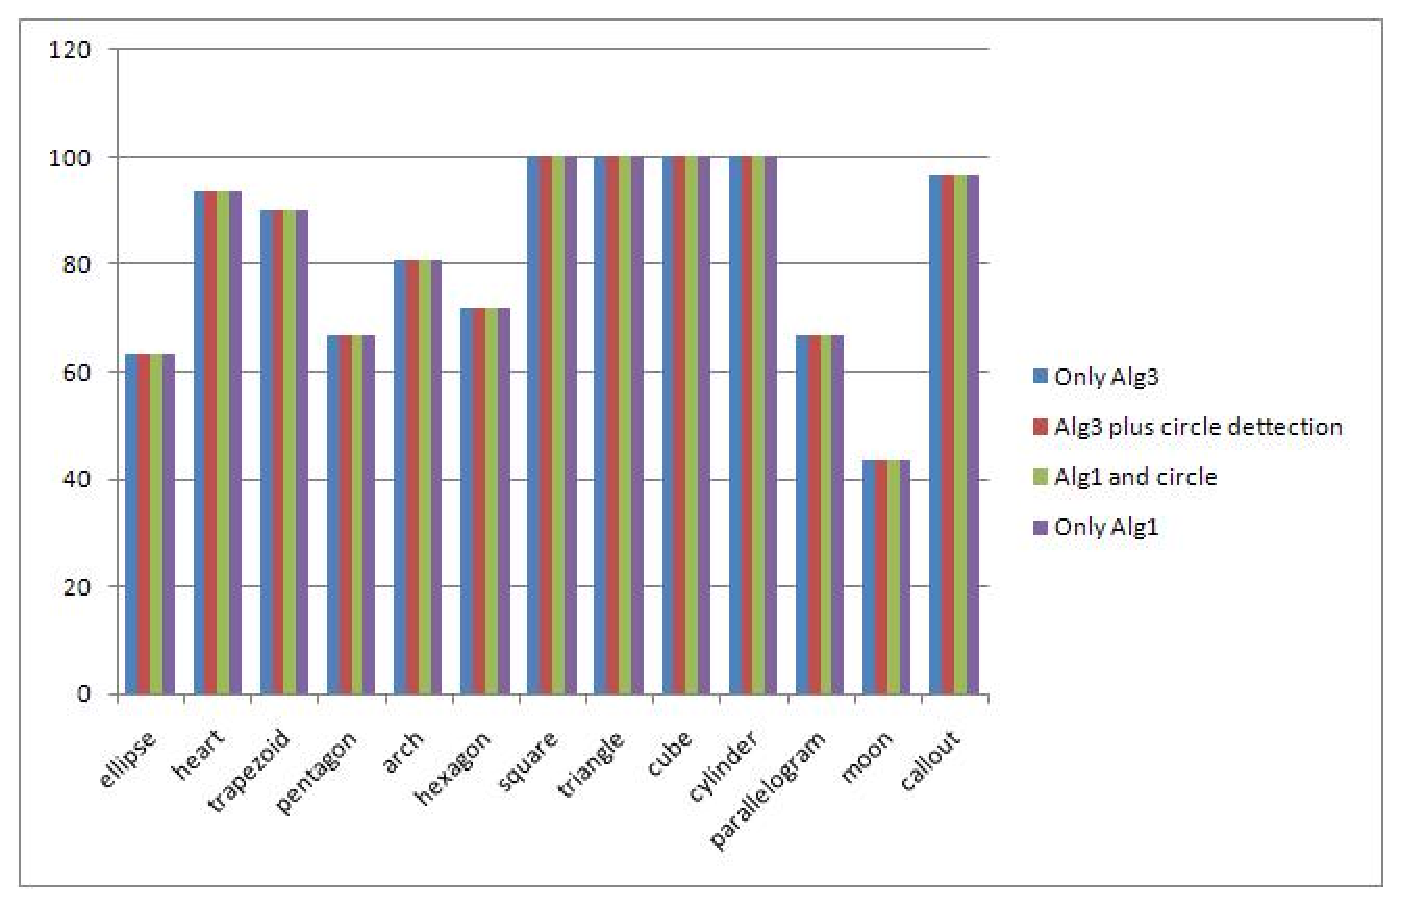
\includegraphics[scale=0.5]{images/test2.eps}
	\caption{The results of second experiment}
	\label{fig:test2}
\end{figure*}
 Another experiment we performed was to test the efficiency svm classifier. We implemented the linear discriminator classifier described in \cite{gestureexample12}(see figure \ref{fig:test3}).  %The result shows that SVM is more scalable than the linear discriminator for this problem. %The test focus on the size of data needed to test each classifier and the achieved accuracy.  %For this experiment we also shows the classification time for both classifiers 
\begin{figure}[]
	\centering
		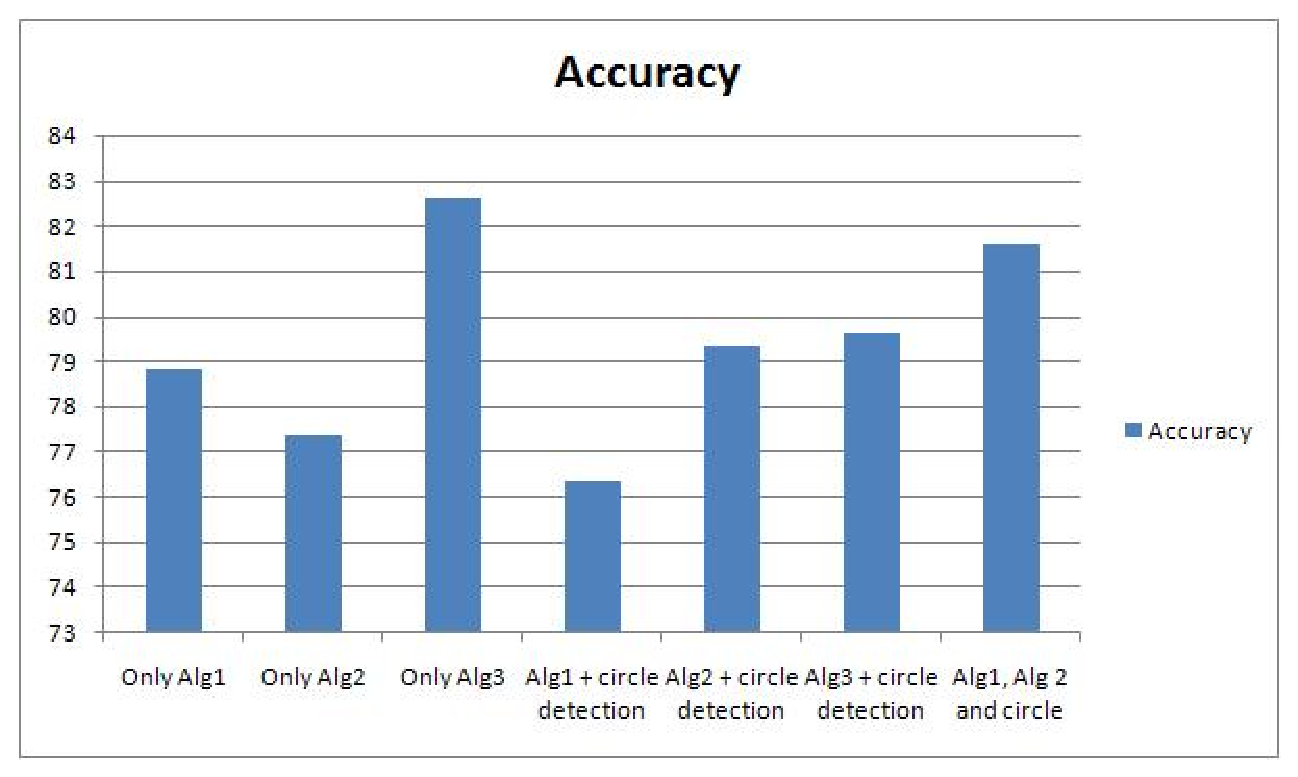
\includegraphics[scale=0.4]{images/test1.eps}
	\caption{The results of third experiment}
	\label{fig:test3}
\end{figure}
 %Details description of results got from comparing various algorithms  
 %Describe data set used for experiments ( No of data set, No. of categories, No of samples).
 %Describe other Algorithms [Alg 3 in paper \cite{earlyprocess}]used for comparing with the one described in the paper. 
 
 %In the figure \ref{fig:test1}, the accuracy means that final hit rate of all symbols used in the test set.by the  four datasets . 
We performed three experiments to test the system firstly we tested recognition accuracy of shapes in the data set with both algorithms. We also implemented the segmentation algorithm described in \cite{earlyprocess} to use as reference to our swarm algorithms.  As you see in the fig. \ref{fig:test1} shows the accuracy achieved by each algorithm. The results shows that both PSO algorithm achieve better result than other algorithms.  The swarm algorithms were tested with and without the ellipse detection module. The ellipse detection module appear to be superior to results with only the PSO algorithms.  \\  
\begin{figure}[]
	\centering
		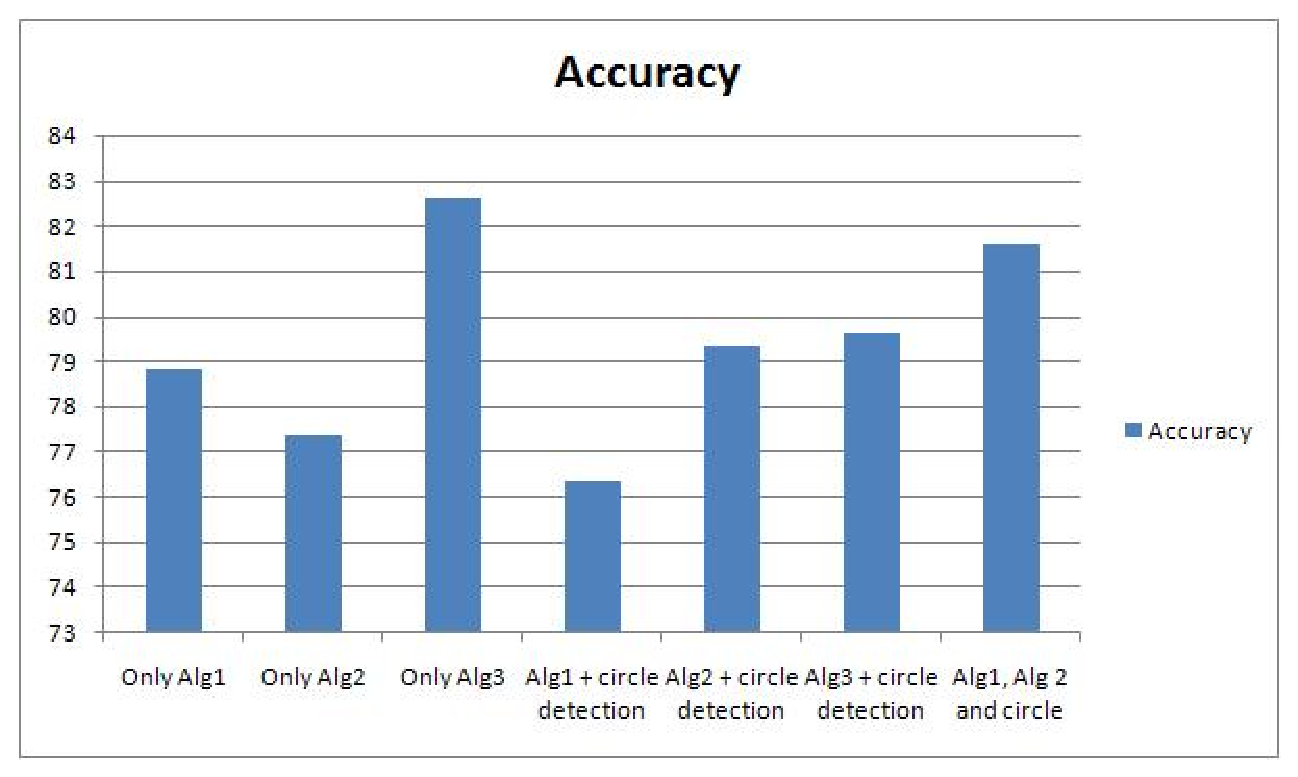
\includegraphics[scale=0.3]{images/test1.eps}
	\caption{The results of first experiment}
	\label{fig:test1}
\end{figure}
 
%\subsection{Clustering Algorithm Results}
%\label{sec:ClusteringAlgorithmResults}

\subsection {Recognition Algorithms }
\label{sec:recognitionAlgorithms}
To test the recognition different set of features are used to select the features that will define symbols better to finally achieve better recognition rate. We tested the system using different types of features. The features explained in section \ref{sec:FeatureExtraction} was divided into different sets; statistical, structural, Rubine features and zernik moments along with composite features. The fig. \ref{fig:testFeatures} shows the result of each set of features when used with the SVM classifier. The results shows that the Rubine features although may achieve good results in single stroke symbols, have a bad performance when used with multi stroke symbols. 
\begin{figure}[]
	\centering
		\includegraphics[scale=0.3]{images/test4.eps}
	\caption{The results of Features experiment}
	\label{fig:testFeatures}
\end{figure}



We test the system using different classifier to see what the effect of the classification step on the final recognition. We also wanted to test the train and test time in both classifiers. We used SVM (RBF) classifiers and the Gaussian Linear classifier used in \cite{}. The fig. \ref{} shows the result of both classifiers with the main three segmentation algorithms. The results shows that the SVM classifier achieve better results. To measure the scalability of the system\footnote{What happens when adding a new symbols to the set of known symbols.} the classifiers are test using different number of symbols (fig. \ref{fig:sampleperCat}). Figures \ref{fig:sampleperCat} demonstrate the scalability of both classifiers by demonstrating the recognition rate in both classifiers with different number of symbols. Figures \ref{fig:sampleperCat},\ref{fig:sampleperCat} shows the time and number of symbols needed for training versus each classifier. 

\begin{figure}
	\centering
		\includegraphics{images/sampleperCat.eps}
	\caption{Samples per Category }
	\label{fig:sampleperCat}
\end{figure}

\begin{figure}
	\centering
		\includegraphics[scale=0.7]{images/test4.eps}
	\caption{Tests}
	\label{fig:test4}
\end{figure}

\section{Summary}
\label{sec:ResultSummary}

The result illustrated in this chapter shows the work done on the system and experiments performed. The results shows that the ellipse detection and PSO swarm algorithms gives better performance than other known systems. 

%\section{ BenchMark Results }
%\label{sec:BenchMarkResults}

